%--------------------------------------------------------------------------------
\documentclass[]{YIC2015}

% --------------------------------------------------------------------------------
% Include here your latex packages
%--------------------------------------------------------------------------------
\usepackage{graphicx}
\usepackage{color}

% --------------------------------------------------------------------------------
% Article's title, with capital letter only at the beginning
%--------------------------------------------------------------------------------
\title{Modeling the I/O behavior of the NEST simulator using a proxy}

% -------------------------------------------------------------------------------
% List of authors
% --------------------------------------------------------------------------------
% Put the initials and surname of the first author ('et al.' if applicable) in
% square brackets before the command \author
%
% Identify the corresponding author with the command \corref and each author
% with the command \authref{a,b,...} according to the affiliation
%
\author[T. Schumann et al.]{%
  T. Schumann\authref{a}\corref,
  W. Frings\authref{b},
  A. Peyser\authref{c},
  W. Schenck\authref{c},
  K. Thust\authref{b},
  J.M. Eppler\authref{c}
}

% --------------------------------------------------------------------------------
% Affiliations
% --------------------------------------------------------------------------------
\address{\authaddr{a}{Institute of Neuroscience and Medicine (INM-6), Computational and Systems Neuroscience \\ %
    Institute for Advanced Simulation (IAS-6) \\ %
    J\"ulich Aachen Research Alliance \\ %
    Forschungszentrum J\"ulich GmbH \\ %
    52425 J\"ulich, Germany}
  \authaddr{b}{J\"ulich Supercomputing Centre \\ %
    Institute for Advanced Simulation \\ %
    Forschungszentrum J\"ulich GmbH\\ %
    52425 J\"ulich, Germany}
  \authaddr{c}{Simulation Lab Neuroscience - Bernstein Facility for Simulation and Database Technology \\ %
    Institute for Advanced Simulation \\ %
    J\"ulich Aachen Research Alliance \\ %
    Forschungszentrum J\"ulich GmbH \\ %
    52425 J\"ulich, Germany}
}
%
% --------------------------------------------------------------------------------
% Email address of the corresponding author
% --------------------------------------------------------------------------------
\corauth{till.schumann@rwth-aachen.de}

% --------------------------------------------------------------------------------
% Abstract
% --------------------------------------------------------------------------------
\abstract{\textit{
NEST \cite{NEST} is a simulator for spiking neural
  networks. It runs on local machines, small clusters and
  supercomputers \cite{Plesser07}. Storing simulation data efficiently
  is essential for neuroscientific studies but is not trivial on
  supercomputers with centralized storage. To assess different I/O strategies and libraries, we have implemented a
  \emph{proxy} which imitates the writing behavior of NEST.  This proxy allows benchmarking and statistical analysis, and
  thus consequent optimizations, without the complexity of running full
  NEST simulations.
}}

% --------------------------------------------------------------------------------
% Keywords - must be separated by semicolon and no capital letters.
% --------------------------------------------------------------------------------
\keywords{parallel I/O; simulation; neuronal networks; supercomputer;
  threading; MPI}

% --------------------------------------------------------------------------------
% Beginning of document
% --------------------------------------------------------------------------------
\begin{document}

\maketitle

% --------------------------------------------------------------------------------
% Beginning of one section
% --------------------------------------------------------------------------------
\section{Introduction}
%
Over the past 20 years, the NEST Initiative \cite{NESTInitiative} has developed the NEST
\cite{NEST} simulator for spiking neural network models. It is used in
computational neuroscience to simulate the dynamics of the interaction
between nerve cells. The systems explored with NEST range from small
networks simulated on local machines up to large brain-scale circuits
using the full capabilities of the world's leading supercomputers. To
have this flexibility, NEST is parallelized in a hybrid fashion
using threads on a compute node and MPI to communicate between the
compute nodes \cite{Plesser07}.  Storing simulation data from such a
massively parallel application efficiently during runtime is essential
for neuroscientic studies, but not a trivial task on a supercomputer
with centralized storage.

Virtual devices store neuronal properties such as spiking activity
and membrane voltage to disk. With increasing numbers of devices and
compute nodes, opening files and writing to them become major bottlenecks, thus requiring
new I/O strategies.

Until now, NEST has used the C++ standard I/O library to store
simulation results to disk.  In the case of large scale simulations on
supercomputers, a huge number of virtual devices can request file
access simultaneously, leading to write system calls becoming a
significant element of overhead. We have therefore investigated
possible performance gains by replacing the current I/O paradigm with
calls to parallelized I/O libraries which could avoid serialization
bottlenecks when interacting with underlying file systems such as GPFS
\cite{GPFS} for highly parallel simulations.

\section{Implement I/O interface}
NEST is used for large variation of use cases.
Therefore different requirements on efficiency and output file formats are required.
To increase the use cases of I/O, an interface is developed which connects the virtual devices with the I/O libraries.
Taking into account that some of the libraries use the MPI layer,
the interface has to contain besides the open, close and write functions, synchronization functions.
The synchronization function allows the usage of inter node communication during simulation.
It has to be guarantied that the synchronization function is called simultaneously on all nodes.

\begin{figure}[htbp]
\centering %
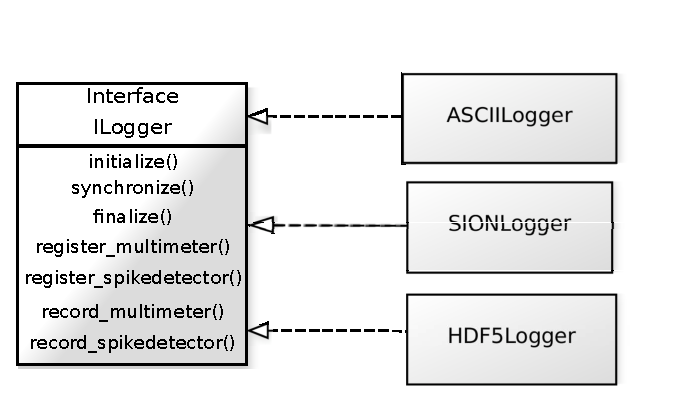
\includegraphics[scale=0.5]{loggerinterface.eps}
\caption{Interface class of the logger}
\label{fig:loggerinterface}
\end{figure}


\subsection{Writing use cases of NEST}
\pleasewrite{Jochen}{the random balanced network and the reduced model of the visual
cortex}

\section{Proxy development}
To develop new I/O strategies information about writing behavior of NEST is necessary.
Therefore the main algorithms of NEST are analyzed and typical writing behavior is estimated.
Taking into account that NEST is a neuronal simulator,
which builds up a network and simulates for each  node equations in dependency of its neighbors,
the program structure only tells information about possible but not the expected writing behavior.
Therefore the code analysis is extended with a runtime measurement which covers standard use cases.

\subsection{Workflow of NESTProxy}
The NESTProxy contains three main parts: Construction of the network, iteration loop and destruction of the network.
In the first part each node creates a set of \emph{Spikedetector} and \emph{Multimeter} objects.
The number is taken from the input parameters \emph{numberOfSpikeDetectorsPerThread} and \emph{numberOfMultimetersPerThread} respectivly.
The objects are initialized with their parameters \ref{tab:table-silva1}
(for \emph{Spikedetector}: \emph{spikesPerDector} and \emph{Multimeter}: \emph{samlpingIntervalsOfMeter}, \emph{numberOfValuesWrittenByMeter}.
The iteration loops contains a sleep function, which uses the distribution from \emph{deadTimeDeliver},
all update function calls of the \emph{Spikedetector} and \emph{Multimeter} object and between this calls 
a sleep function, which uses the distribution from \emph{deadTimeUpdate}.
During the update function each \emph{Spikedetector}, \emph{Multimeter} object calls one or multiple write function, depending on its distribution variable.


\subsection{Analyze NEST code}
The algorithms of NEST are globally time-driven with constant time steps.
In each time step all neurons are updated iteratively.
The main program structure can be reduced to a for loop of update functions of neurons.
In the update function neurons call their own algorithm, which may contain writing calls.
Whether a writing call occurs depends on the algorithm and the whole neuronal network structure.
Because of a weight variation of algorithms and neuronal network structures, the update function is considered a black box.
Statistical values shell be used to reproduce the occurrence of writing calls in the update functions.

\subsection{Measure NEST runtime behavior}
To generate reliable timing mesaurements of the runtime behavior,
the NEST code is instrumented with ScoreP \cite{scoreP}.
\pleasewrite{Wolfram}{Scorep analysis}
Resulting runs of the instrumented NEST,
produce time series of function calls for standard use cases.
Only functions are instrumented, which have an potencial influence on the writing behavior.
This time series are used to estimate the distribution of the timings.

\begin{table}[htdp]
\caption{Stochastical parameters, which are input parameters of the NESTProxy}
\centering
\begin{tabular}{lll}
\hline\hline
\textbf{Type} & \textbf{Name} & \textbf{Description} \\ \hline
Integer &   numberOfSpikeDetectorsPerThread & number of SpikeDetectors per thread  \\
Integer &   numberOfMultimetersPerThread & number of Multimeters per thread  \\
Distribution &   spikesPerDector & number of spikes generated at each SpikeDetector per iteration  \\
Distribution &   samlpingIntervalsOfMeter & sampling interval of the Multimeters  \\
Distribution &   numberOfValuesWrittenByMeter & number of written values by each Multimeter in sampling interval  \\
Distribution  &  deadTimeUpdate & sleeping timings between SpikeDetector and Multimeters writing operations \\
Distribution &   deadTimeDeliver & sleeing time in deliver function  \\
\hline\hline
\end{tabular}
\label{tab:table-silva1}
\end{table}


\section{Implement drivers}
Based on the interface descripted above different drivers are
implemented.

\subsection{ASCII}
Current versions of NEST use the standard C++ IO Stream library
\cite{stream} to permanently store results as plain text files
containing such information as time stamps as floating point
strings. The advantage of such a scheme is simplicity in
implementation and in post-processing for analysis in addition to
plain-text's self-descriptive nature.

However for large-scale simulations, this leads to: 1) excessively
large amounts of data written to disk which is both a performance
issue and a practical storage problem; 2) a serialization bottleneck
when opening a separate file per process; and 3) a serialization
bottleneck for metadata updates in the file system when new blocks are
allocated. One solution used in recent iterations of NEST has been the
implementation of a global spike detector \cite{gsd}: a single file is
opened by rank 0 to store spiking events, a low cost solution since
currently all ranks see all spike events through MPI collective
communication. On the other hand, such an approach has several
long-term consequences: 1) it constitutes a serialization bottleneck
as spike event I/O is handled by only a single rank rather than being
distributed over available processors; 2) it is a design constraint,
depending upon all spikes being globally shipped which may not be
scalable; and 3) it is inapplicable to more voluminous data such as
membrane potential measurements which can not be tractably shipped to
a single I/O node.

We will use an ``ASCII'' driver, though, as a benchmark to compare
other approaches, as a robust backup for debugging and validating
other drivers, and as a legacy interface allowing backwards
compatibility. This requirement has required us to begin abstracting
the current interface to a common API in the context of SIONLIB and
HDF5 interfaces.

\subsection{SIONLIB}
\pleasewrite{Kay}{sionlib advantages}

\subsection{HDF5}
HDF5 is an API to commonly used file formats in the neuroscience
community, such as NEON \cite{neon} and Neuroshare \cite{neuroshare}.
Since they use a common binary layout and API, data can be accessed
from many different languages and through many different libraries. In
particular, the HDF group publishes pHDF5 (parallel HDF5,
\cite{phdf5}) which allows read and write access to HDF5 file formats
over MPI connected networks with tuning for particular HPC file
systems such as Luster. 

HDF5 is not a streaming file format, but a highly structured,
self-describing format intended for long-term accessibility and
versatile usage. The cost of this is that significant amounts of
metadata must be stored to describe the data layout, creating a
collective barrier when finite data structures are extended, as we
have when additional unpredictable spiking event data must be stored,
or the length of a simulation is extended for continuous data
acquisition. In short, pHDF5 is read-oriented rather than
write-oriented, with some of the same drawbacks (and advantages) for
writing seen with the ASCII driver.

Therefore, for large neuronal networks simulated in NEST, we have
found it difficult to produce performance similar to what we have done
with SIONLIB. 

\section{Benchmarking and statistical analysis}


\section{CONCLUSIONS}
The presented IO interface for NEST forms the flexibility to implement varies IO libraries independently.
To optimize the implemented IO library the NESTProxy allows simple benchmarking without the overhead of the whole NEST program.
The development of the IO libraries can be done separately from NEST.
Taking into account that NEST is one of the leading neuronal simulators, which run on the fastest super computers available,
the NESTProxy can be used as a benchmarking tool for parallel IO libraries.

\section*{ACKNOWLEDGEMENTS}
Enter acknowledgements directly before the references. Use the format of primary section headers, but do not number the acknowledgement and references sections.


% --------------------------------------------------------------------------------
% Bibliography
% --------------------------------------------------------------------------------
\begin{thebibliography}{99}

% -------------------------------------------------------------------------------
% Bibliography - example of book's reference
% -------------------------------------------------------------------------------
\bibitem{bookref} %
F.~Author, S.~Author, T.~Author. \textit{Title}. Publisher, Year.

% --------------------------------------------------------------------------------
% Bibliography - example of journal's reference
% --------------------------------------------------------------------------------
\bibitem{NEST} %
M.~Gewaltig, M.~Diesmann. \{NEST\} (\{NE\}ural \{S\}imulation \{T\}ool). \textit{Scholarpedia} %
\textbf{2}:1430, 2007.

% --------------------------------------------------------------------------------
% Bibliography - example of proceedings' reference
% --------------------------------------------------------------------------------
\bibitem{Plesser07}
H.~Plesser, J.~Eppler, A.~Morrison. Efficient Parallel Simulation of Large-Scale
                  Neuronal Networks on Clusters of Multiprocessor
                  Computers. In: \textit{Euro-Par 2007: Parallel Processing}, Berlin, Germany, 2007.
                  
\bibitem{frings2009scalable}
W.~Frings, F.~Wolf, V.~Petkov. Scalable massively parallel I/O to task-local files
 In: \textit{High Performance Computing Networking, Storage and Analysis, Proceedings of the Conference on}, Berlin, Germany, 2009.

% --------------------------------------------------------------------------------
% Bibliography - the end.
% --------------------------------------------------------------------------------

\end{thebibliography}

% --------------------------------------------------------------------------------
% End of document
% --------------------------------------------------------------------------------
\end{document}
